\documentclass[11pt, letterpaper]{article}

\usepackage[margin=1in]{geometry}
\usepackage{graphicx}
\usepackage{listings}
\usepackage{xcolor}
\usepackage{booktabs}
\usepackage{hyperref}
\usepackage{titlesec}
\usepackage{parskip}
\usepackage{fancyhdr}
\usepackage{caption}

% ── Header / footer ──────────────────────────────────────────────────────────
\pagestyle{fancy}
\fancyhf{}
\lhead{\small EECE 5155 -- Take-Home Task 1}
\rhead{\small Aiisha Matsungo}
\cfoot{\thepage}
\renewcommand{\headrulewidth}{0.4pt}

% ── Section formatting ────────────────────────────────────────────────────────
\titleformat{\section}{\large\bfseries}{}{0em}{}[\titlerule]
\titleformat{\subsection}{\normalsize\bfseries}{}{0em}{}

% ── Code listings ─────────────────────────────────────────────────────────────
\lstset{
  basicstyle=\ttfamily\small,
  backgroundcolor=\color{gray!8},
  frame=single,
  framerule=0.4pt,
  rulecolor=\color{gray!40},
  breaklines=true,
  xleftmargin=8pt,
  xrightmargin=8pt,
  aboveskip=6pt,
  belowskip=6pt,
}

% ─────────────────────────────────────────────────────────────────────────────
\begin{document}

\begin{center}
  {\LARGE\bfseries Task 1: Extended Grafana Dashboard}\\[6pt]
  {\large EECE 5155 -- Wireless Sensor Networks and IoT Systems}\\[4pt]
  {\normalsize Aiisha Matsungo \quad|\quad NUID: 002530298 \quad|\quad March 2026}
\end{center}
\vspace{4pt}\hrule\vspace{10pt}

% ─────────────────────────────────────────────────────────────────────────────
\section{Overview}

The seminar 4 panels dashboard using the
\texttt{iot-sensors} InfluxDB bucket populated during the seminar via the
MQTT publisher and bridge pipeline. All queries use Flux and target the
IoT temperature dataset (Kaggle, 97,606 rows, Oct--Dec 2018).

% ─────────────────────────────────────────────────────────────────────────────
\section{Final Dashboard Screenshot}

\begin{figure}[h]
  \centering
 
  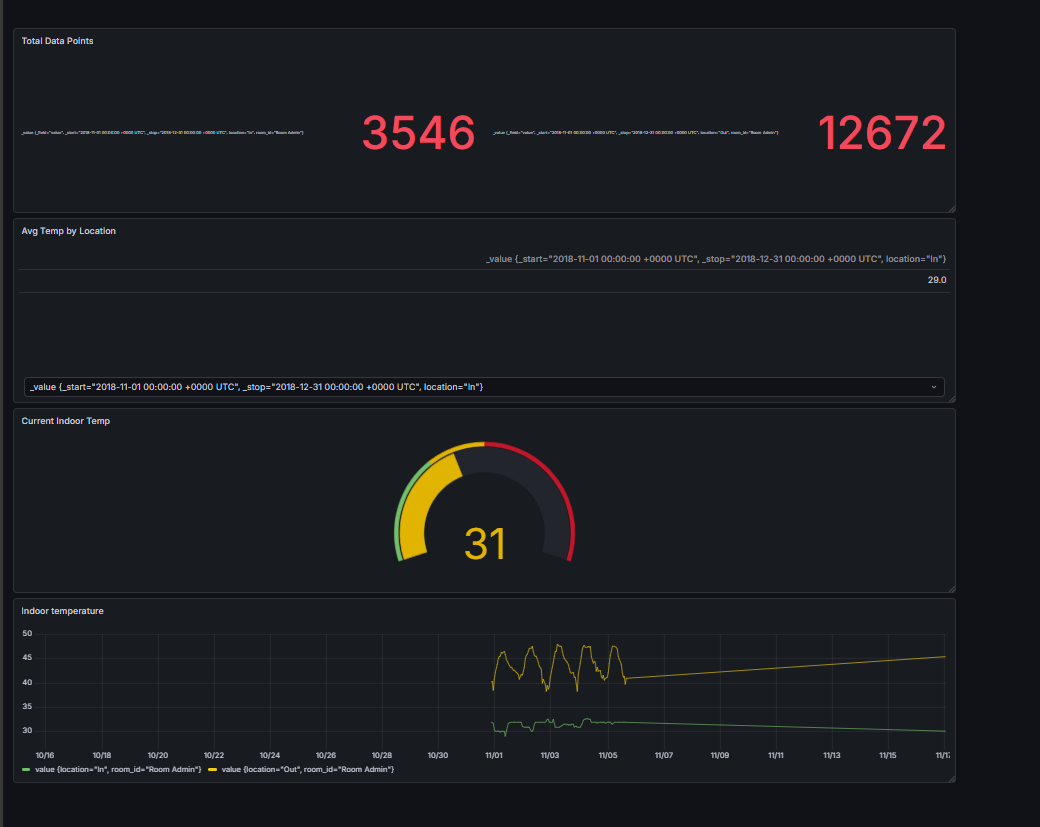
\includegraphics[width=\textwidth]{dashboard.png}
  \caption{4-panel Grafana dashboard -- IoT Seminar, \texttt{iot-sensors} bucket}
\end{figure}

% ─────────────────────────────────────────────────────────────────────────────
\section{Panel Descriptions and Flux Queries}

\subsection{Panel 1 -- Total Data Points (Stat)}

Displays the total count of ingested readings split by indoor and outdoor location.
Two Stat values are shown side by side: 3,546 (Indoor) and 12,672 (Outdoor).

\begin{lstlisting}[caption={Panel 1 -- Indoor count}]
from(bucket: "iot-sensors")
  |> range(start: 2018-10-01T00:00:00Z, stop: 2018-12-31T00:00:00Z)
  |> filter(fn: (r) => r._measurement == "temperature")
  |> filter(fn: (r) => r._field == "value")
  |> filter(fn: (r) => r.location == "In")
  |> count()
\end{lstlisting}

\begin{lstlisting}[caption={Panel 1 -- Outdoor count (second query)}]
from(bucket: "iot-sensors")
  |> range(start: 2018-10-01T00:00:00Z, stop: 2018-12-31T00:00:00Z)
  |> filter(fn: (r) => r._measurement == "temperature")
  |> filter(fn: (r) => r._field == "value")
  |> filter(fn: (r) => r.location == "Out")
  |> count()
\end{lstlisting}

% ── Panel 2 ──────────────────────────────────────────────────────────────────
\subsection{Panel 2 -- Avg Temp by Location (Table)}

Displays the mean temperature for Indoor (29.0\,°C) and Outdoor locations
over the Nov--Dec 2018 window.

\begin{lstlisting}[caption={Panel 2 -- Average temperature grouped by location}]
from(bucket: "iot-sensors")
  |> range(start: 2018-11-01T00:00:00Z, stop: 2018-12-31T00:00:00Z)
  |> filter(fn: (r) => r._measurement == "temperature")
  |> filter(fn: (r) => r._field == "value")
  |> group(columns: ["location"])
  |> mean()
\end{lstlisting}

% ── Panel 3 ──────────────────────────────────────────────────────────────────
\subsection{Panel 3 -- Current Indoor Temp (Gauge)}

Shows the most recent indoor temperature reading as a colour-coded gauge.
Thresholds: green $<$28\,°C, yellow 28--35\,°C, red $\geq$35\,°C.
Current reading: \textbf{31\,°C} (yellow -- warm but within tolerance).
Threshold mode set to \textbf{Absolute} (not Percentage) to ensure correct
colour mapping.

\begin{lstlisting}[caption={Panel 3 -- Last indoor temperature reading}]
from(bucket: "iot-sensors")
  |> range(start: 2018-10-01T00:00:00Z, stop: 2018-12-31T00:00:00Z)
  |> filter(fn: (r) => r._measurement == "temperature")
  |> filter(fn: (r) => r._field == "value")
  |> filter(fn: (r) => r.location == "In")
  |> last()
\end{lstlisting}

% ── Panel 4 ──────────────────────────────────────────────────────────────────
\subsection{Panel 4 -- Indoor Temperature Over Time (Time Series)}

Time-series chart showing hourly mean temperature for both Indoor (green,
$\approx$30--32\,°C) and Outdoor (yellow, 38--47\,°C with visible daily
cycling Oct--Nov, stabilising after Nov 5). The outdoor oscillation pattern
reflects natural diurnal variation; the flattening after Nov is an artefact
of the aggregation window smoothing fewer data points.

\begin{lstlisting}[caption={Panel 4 -- Hourly aggregated time series}]
from(bucket: "iot-sensors")
  |> range(start: 2018-10-15T00:00:00Z, stop: 2018-11-17T00:00:00Z)
  |> filter(fn: (r) => r._measurement == "temperature")
  |> filter(fn: (r) => r._field == "value")
  |> aggregateWindow(every: 1h, fn: mean)
\end{lstlisting}

% ─────────────────────────────────────────────────────────────────────────────
\section{AI Audit}

\textbf{What AI got right:}
Suggested a Stat panel using \texttt{count()} and a Table panel using
\texttt{group(columns: ["location"]) |> mean()} -- both were relevant and ran
correctly after pasting into the Flux editor.

\textbf{What AI got wrong / what I fixed:}
The initial queries used \texttt{range(start: -30d)} which returned no data
because the dataset is from 2018. I changed the time range to a hardcoded
absolute range (\texttt{2018-10-01} to \texttt{2018-12-31}).
The gauge also displayed all red initially because Threshold mode defaulted
to \textbf{Percentage} instead of \textbf{Absolute} -- fixed in the panel options.

% ─────────────────────────────────────────────────────────────────────────────
\section{What I Learned}

Grafana's \texttt{range(start: -30d)} is relative to \textit{now}, so historical
datasets return empty unless you hardcode absolute timestamps or set the dashboard
time picker to match the data's actual date range.
I also learned that gauge thresholds default to Percentage mode -- at 28 and 35
on a 15--55 scale, percentage mode placed the boundaries at $\approx$26\,°C and
$\approx$29\,°C, collapsing the yellow band almost entirely and making 31\,°C
appear red. Switching to Absolute fixed the colour mapping immediately.
More broadly, visualisation type matters: the same mean-by-location query reads
as a single number in Table view but becomes immediately comparable in Bar chart
view -- choosing the right panel type is as important as writing the correct query.

\end{document}
